        \clearpage
        \begin{figure*}[ht]
            \pdfbookmark[2]{ID 06}{figure_id_06}
        	\centering
            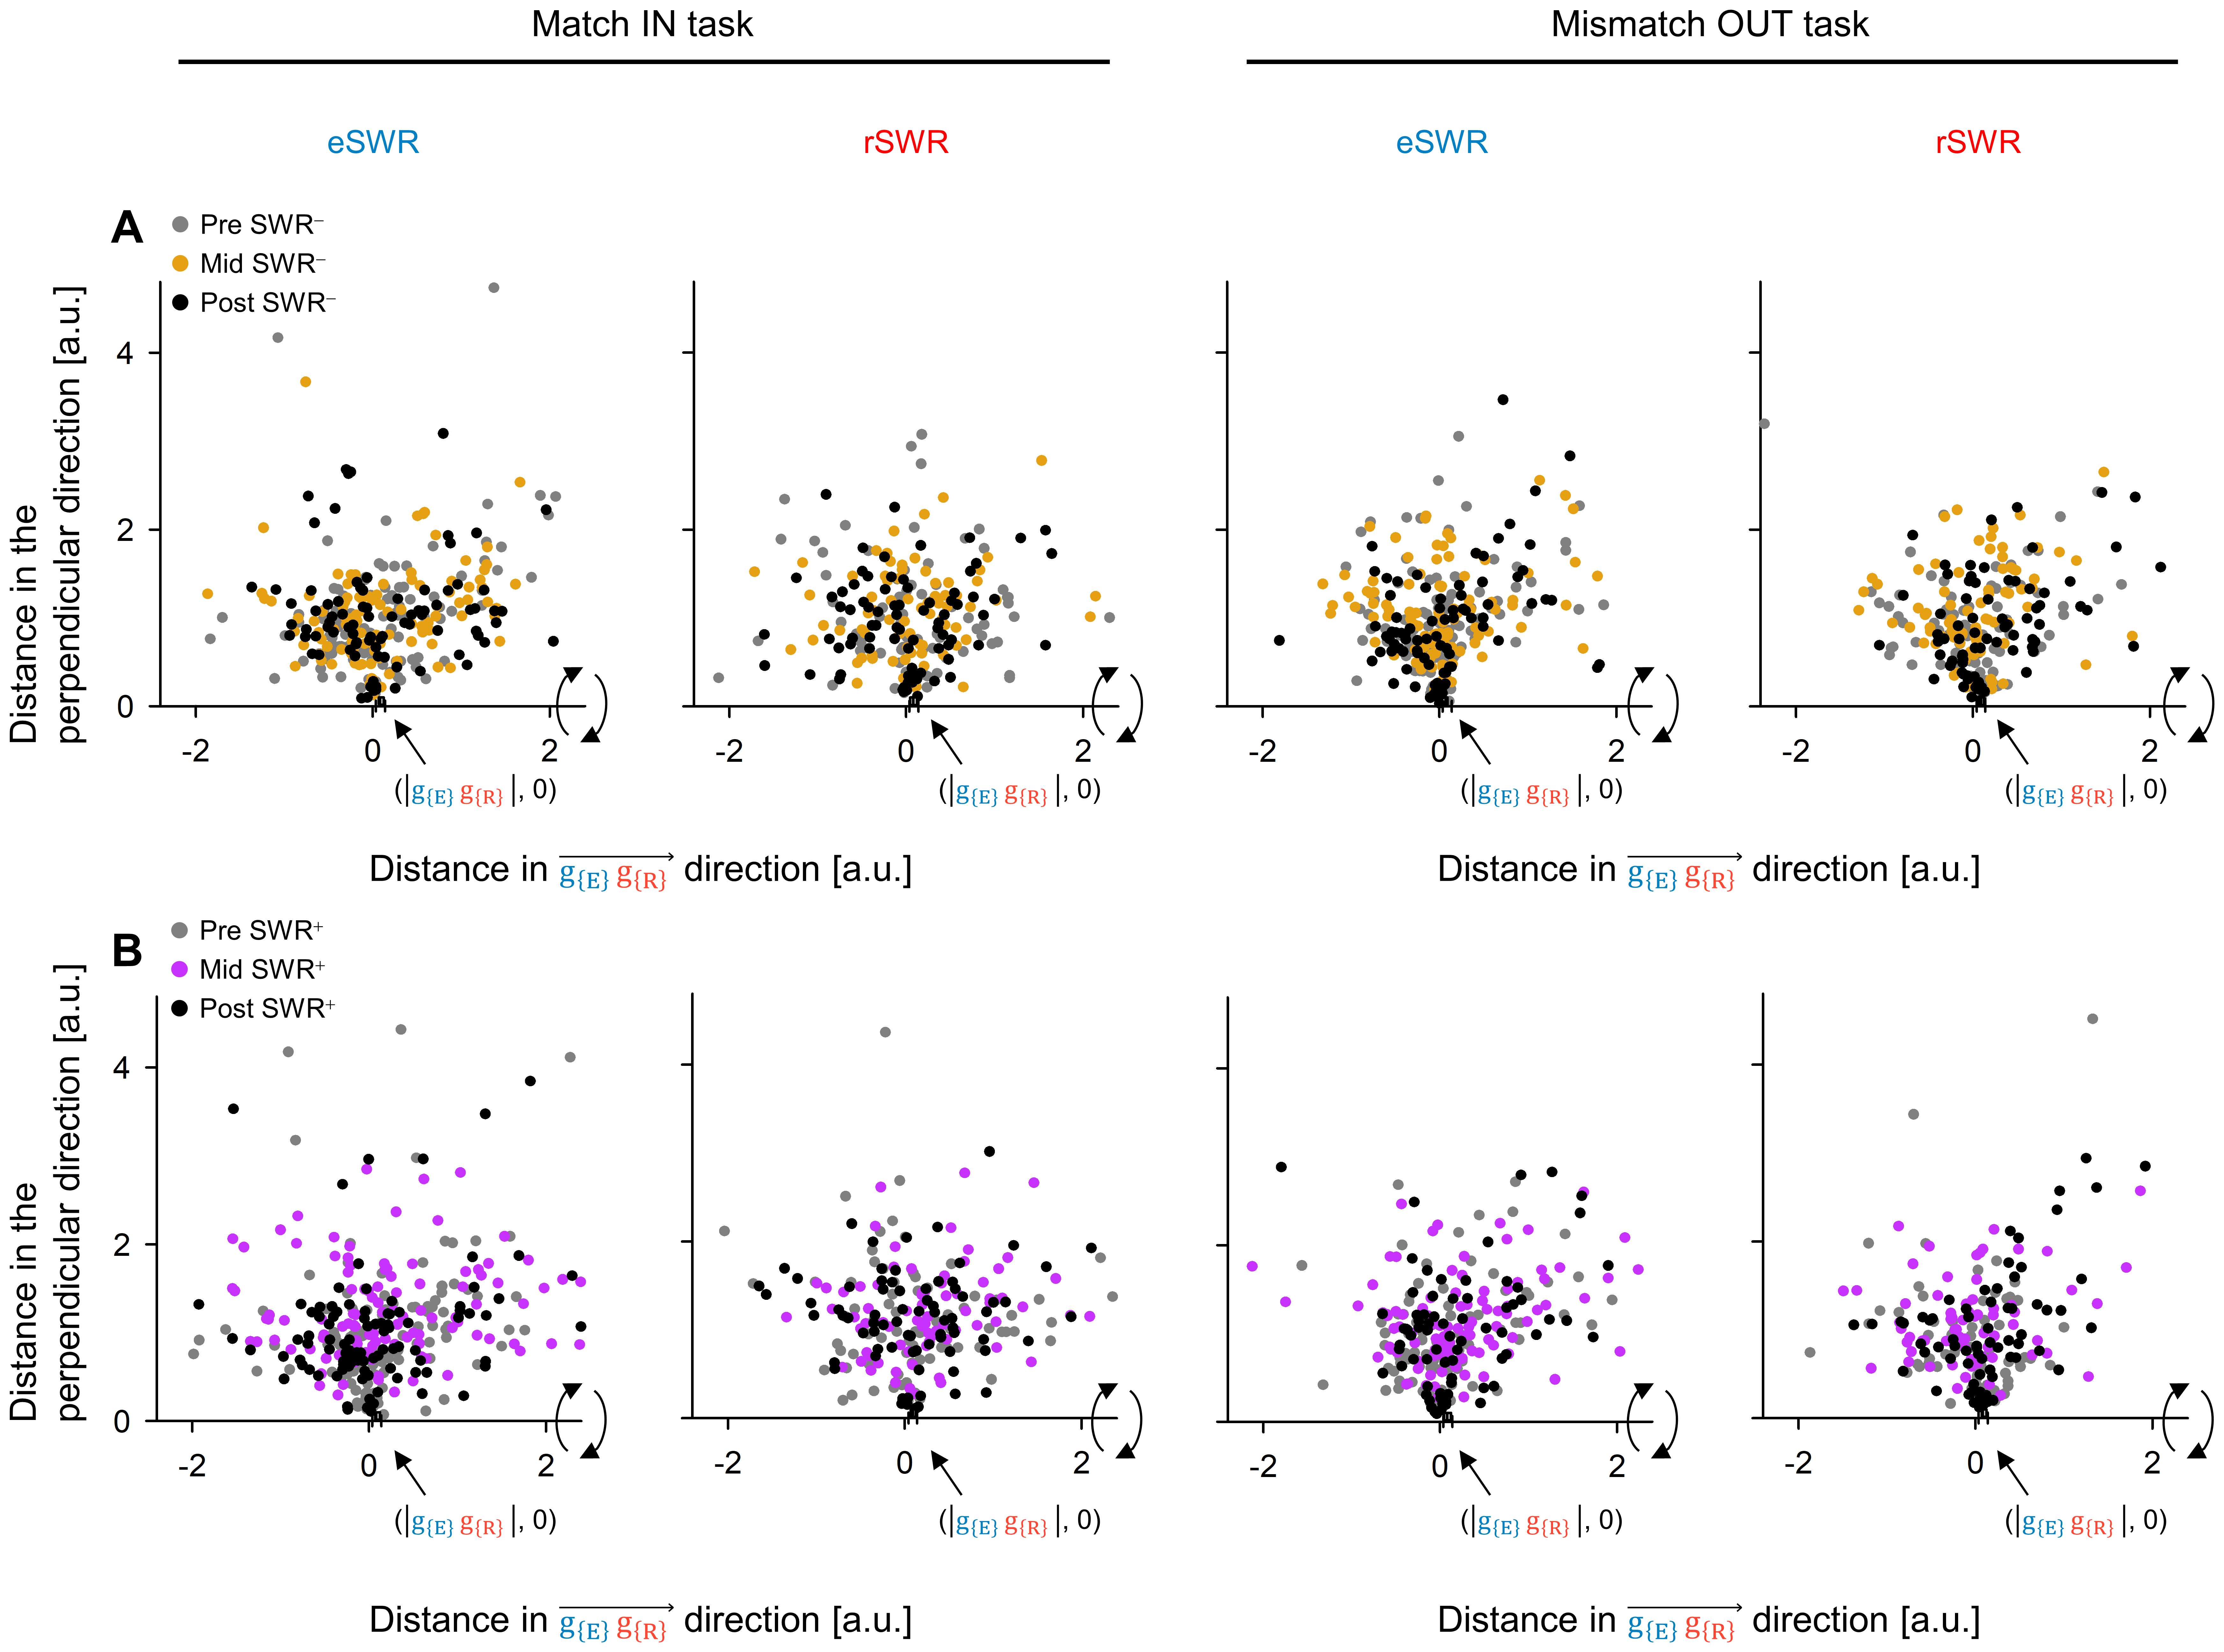
\includegraphics[width=1\textwidth]{./src/figures/.png/Figure_ID_06.png}
        	\caption{\textbf{Visualizing Neural Trajectories During Sharp-Wave Ripple Events in a Two-Dimensional Space}

\smallskip

\\
This illustration showcases neural trajectories association with hippocampal activity during Sharp-Wave Ripple (SWR) events, as displayed in a two-dimensional context. \textbf{\textit{A.}} It presents exemplar trajectories of the pre- (\textit{gray}), mid- (\textit{yellow}), and post-SWR$^-$ (\textit{black}) phases of an SWR event~\cite{buzsaki_hippocampal_2015}. \textbf{\textit{B.}} Shown here are the trajectories that align with SWR$^+$ circumstances, as observed against the SWR$^-$ backgrounds~\cite{fernandez-ruiz_long-duration_2019}. The magnitude of $\lVert \mathrm{g_{E}g_{R}} \rVert$ displays patterns of variation across sessions~\cite{liu_consensus_2022}. The projection protocol can be described as follows: initially, $\mathrm{g_{E}}$ was positioned at the origin $O$ (0,0), and $\mathrm{g_{R}}$ at ($\lVert \mathrm{g_{E}g_{R}} \rVert$, 0), achieved through linear transformation~\cite{kim_corticalhippocampal_2022}. Later, a rotation of the point cloud around the $\mathrm{g_{E}g_{R}}$ axis (the x-axis) was performed, allowing compatibility with a two-dimensional space~\cite{yu_gaussian-process_2009}. Consequently, both the distances from $O$ and the angles relative to the $\mathrm{g_{E}g_{R}}$ axis maintained the same attributes as in their three-dimensional arrangement~\cite{mcinnes_umap_2018}. Acronyms and terms used: SWR refers to Sharp-Wave Ripple events; eSWR stands for SWR during the encoding phase; rSWR indicates SWR during the retrieval phase; SWR$^+$ represents an SWR event; SWR$^-$ designates the control event for SWR$^+$; the terms pre-SWR, mid-SWR, and post-SWR delineate the time intervals ranging from $-800$ to $-250$ ms, from $-250$ to $+250$ ms, and from $+250$ to $+800$ ms from the center of an SWR event, respectively~\cite{zhang_hippocampal_2022}.
}
% width=1\textwidth
        	\label{fig:06}
        \end{figure*}
